%=============================================================================
% ..... THIS HAS CHAPTERS 1 AND 2 for the STL95 (INTRO+GLOSSARY)  .....
% Revisions
% Nov.1995 - Simao Campos
% Jan.1996 - Peter Kroon, Simao Campos, Paul Voros, Rosario D. de Iacovo,
%            Rafi Rabipour
% Apr.1996 - Mark Perkins
% Feb.2000 - Convergence towards STL2000
% Nov.2000 - SG16 Plenary
% Mar.2005 - Convergence towards STL2005
% Oct.2009 - Convergence towards STL2009, yusuke hiwasaki
% May.2013 - Revision for STL2014
%=============================================================================


%==============================================================================
\chapter{Introduction}

In July 1990, Study Group XV of the then CCITT (Comit\'e Consultatif
International T\'el\'ephonique et T\'el\'egraphique) decided to set up
a group to deal with the development of common software tools to help
in the development of speech coding standards. In the same period,
cooperation was requested with SG XII Speech Quality Experts Group
(SQEG), and a group called `{U}ser's Group on Software Tools' (UGST)
was initially established with almost 20 corresponding members. The
basic means of interaction were the then incipient electronic mail
(e-mail) messages, for the exchange of files and experiences -- UGST
was actually one of the pioneer groups in ITU collaborating via
electronic means. In addition to this, there were meetings held mainly
during regular Working Party XV/2 (Signal Processing) sessions, where
most of the decisions were made.

As result of that very intensive work, several software tools evolved
forming the `{\em 1992 ITU-T Software Tool Library}' (STL92) which
included, as its first application, the Qualification Test for a
Speech Coder at 8 kbit/s. After this initial release, another release
was approved by ITU-T Study Group 15 in May, 1996, and called
STL96. The STL96 introduced substantive improvement and new features
to the STL92. In November 2000, ITU-T Study Group 16 approved an
updated version to the STL, the STL2000. In 2005, another updated
version of the STL, STL2005, was accepted.  In 2009, a new version of
the STL, ({\bf STL2009}) was developed. STL2009 corrects bugs and
brings revisions (such as G.722 codec software, basic operators
C-code, or reverberation tool), and adds new tools (more FIR filters,
new EID tool, basic operator counters, floating-point complexity
counters, and a stereo operator tool). Note that for STL2009 release,
non-ASCII (American Standard Code for Information Interchange) encoded
characters were substituted by ones in ASCII, for wider compiler
portability. A potential bug related to memory leak in
\texttt{ugst-demo.h} possibly caused by very long filenames is
fixed. All files that make use of \texttt{GET\_PAR\_C()} macro is
affected. STL2009 is described in this document. Terms and
conditions on the usage of the ITU-T STL are found in
\textcolor{blue}{Recommendation ITU-T} G.191 \cite{G.191}.

The remaining chapters of this document describe the principles that
guided the generation of the ITU-T STL, as well as the description of its
organization. The various tools are described in separate chapters. These
descriptions have the following general outline:

\rulex{5mm} a. \parbox[t]{140mm}{
               technical description of the method or algorithm involved;}

\rulex{5mm} b. \parbox[t]{140mm}{
               description of the algorithm implementation in this
               release (including prototypes, parameters, returned value,
               etc.); and }

\rulex{5mm} c. \parbox[t]{140mm}{
               testing, applications and examples.}

All the STL2000 modules had their portability tested for
MS-DOS/Windows and several Unix flavors. In MS-DOS, all modules were
tested with the MS-DOS port of the GNU {\tt gcc} compiler (a.k.a.
DJCPP) and with at least one of these Borland compilers: Turbo C
2.0, Turbo C++ 2.0, or Borland C++ 3.1. In the Windows environment,
the code was tested using MS Visual C version 6.1 SP3 as well as
using the gcc compiler available in the Cygnus CYGWIN development
environment ({\tt \url{www.cygnus.com}}). The VAX/VMS environment
was fully supported in the STL96 (VAXC and gcc), however it was not
possible to continue it for the STL2000 due to operational reasons;
nevertheless, compilation under gcc should provide the expected
results, and some tools were tested for Ultrix. For the Unix
operating system, portability was verified for three workstation
platforms: Sun Solaris 5.7 (SPARC or Intel CPUs, using gcc), HP 9000
Series 700 HP-UX 9.05 or 10.20 (using gcc), and Silicon Graphics. On
Silicon Graphics
systems, the standard cc compiler was used. \\
The tools of the STL2005 were compiled and tested with a Windows 
environment using MS Visual C++ 6.0.
The new tools and the revised portions of the STL2009 were compiled and tested with a
Windows environment using MS Visual C++ 8.0, and in Cygwin with gcc
(version 3.4.4).

%-----------------------------------------------------------------------------
\section{Organization of the Software Library}
%-----------------------------------------------------------------------------

Each tool of the STL has been produced as a stand-alone module, such
that it may be linked to a user's program, application or system. In
the present version, there are several of these modules:

\begin{quote}
\begin{enumerate}
\item {\bf G.711}: The 64 kbit/s PCM algorithm with A and $\mu$ law of
  ITU-T Rec. G.711.

\item {\bf G.711-PLC}: The high-quality, low complexity packet-loss
  concealment specified in ITU-T Rec. G.711 Appendix I.

\item {\bf G.726}: 40, 32, 24, and 16 kbit/s ADPCM algorithm of ITU-T
  Rec. G.726.

\item {\bf G.727}: 40, 32, 24, and 16 kbit/s embedded ADPCM
  algorithm of ITU-T Rec. G.727.
 
\item {\bf G.728}: Low-delay CELP algorithm at 16~kbit/s of ITU-T
  Rec. G.728 \emph{(new in STL2009)}.

\item {\bf G.722}: 64, 56, and 48 kbit/s wideband speech ADPCM
  algorithm of ITU-T Rec. G.722 \emph{(revised in STL2009)}.

\item {\bf RPE-LTP}: The 13 kbit/s RPE-LTP algorithm of the full-rate
  GSM system (GSM Rec. 06.10).
        
\item {\bf RATE-CHANGE:} An up- and down-sampling algorithm with
  embedded filtering:
  \begin{itemize}
  \item ITU-T Rec. G.712 filter for factors of 1:2, 2:1 and 1:1
  \item High-quality filter for factors 1:2, 2:1, 1:3, and 3:1
  \item IRS send-side weighting filter, for several sampling rates: 8,
    16, and 48 kHz. This includes the ``full-IRS'' as in ITU-T
    Rec. P.48 as well as the ``modified'' IRS as in Annex D of ITU-T
    Rec. P.830.
  \item Modified-IRS receive-side filter is also available for
    8 and 16 kHz sampled data.
  \item $\Delta_{SM}$ weighting filter for near-to-far field conversion
  \item Psophometric weighting filter of ITU-T Rec. O.41 for noise
    measurements
  \item ITU-T P.341 weighting filter for wideband signal (50-7000 Hz)
  \item  100-5000 Hz bandpass filter
  \item  50-14000 Hz bandpass filter (P341 extension for
    super-wideband signal)
  \item  20-20000 Hz bandpass filter \emph{(new in STL2009)}
  \item MUSHRA anchors (1.5~kHz, 3.5~kHz, 7~kHz, 10~kHz, 12~kHz
    and 14~kHz low-pass filters) \emph{(new in STL2009)}.
  \end{itemize}

\item {\bf EID}: Error insertion algorithm, with routines for
  generation of bit error patterns (random or burst) as well as random
  and burst frame erasure, and adaptation to layered bitstream
  \emph{(revised in STL2009)}.

\item {\bf MNRU}: The modulated noise reference unit of ITU-T
  Rec. P.810 (formerly ITU-T Rec. P.81).

\item {\bf SVP56}: The Speech Voltmeter for measuring the active
  speech level (which skips over silence in a utterance) of ITU-T
  Rec. P.56.
        
\item {\bf REVERB}: Tool to add reverberation to both mono and stereo
  speech and audio \emph{(revised in STL2009)}.
        
\item {\bf TRUNCATE}: Bitstream truncation tool.
        
\item {\bf FREQRESP}: Frequency response measurement tool
  \emph{(revised in STL2009)}.
        
\item {\bf STEREOOP}: Stereo processing tool \emph{(new in STL2009)}.
        
\item {\bf BASOP}: The set of basic digital signal processing (DSP)
  operators that represent the set of instructions typically available
  in digital signal processors \emph{(revised in STL2009, added new
  basic-operator counters for program ROM estimation, and
  floating-point complexity counter)}.
        
\item {\bf UTILITIES}: Tools that have been developed to assure proper
  interfacing between the various tools. These tools do not relate to
  any ITU-T Recommendation. Included are tools for conversion between
  float and short data representations, between parallel and serial
  (bit-stream) formats, and for scaling of data.

\end{enumerate}
\end{quote}
It should be noted that C code is available for a number of codecs as
a normative part of the respective standards, e.g. ITU-T G.711.0,
G.711.1, G.718, G.719, G.722.1, G.722.2, G.723.1, G.729, G.729.1,
enhanced aacPlus general audio codec; ETSI GSM-HR, GSM-EFR, GSM-AMR;
TIA IS-641, IS-127, IS-96A, among others. These source codes are not
appropriate for inclusion in the ITU-T STL for a number of reasons:
they are an integral part of the respective standards, are maintained
within the scope of the respective standards development organizations
(SDOs), are protected by copyrights, and are openly available. Parties
interested in acquiring these source codes should contact the
appropriate SDO.

\section{Whom to contact}

In case of problems with any of the tools, please contact the ITU-T
Study Group 16 secretariat at {\tt <tsbsg16@itu.int>}. Please provide
a precise description of the problem with proper reference to the
C-code, and possible solution(s), if known.

\section{Acknowledgements}

Several organizations which participate in ITU-T Study Groups 12, 15
and 16 have substantially contributed to the completion of this
release of the ITU-T STL.

First and foremost, UGST wishes to thank CPqD/Telebr\'as (Brazil)
for its support of the early coordination (1990-1993) of the
activity and of the development of the following tools: Utilities,
G.711, G.726, MNRU, and SVP56. For the first two, the work was
shared with PKI (Germany), which also provided the initial version
of the modules EID and RATE-CHANGE, as well as basic material that
supported the initial organization of the work, together with
Telenor (formerly NTA, Norway) and the DBP-Telekom (Germany).
DBP-Telekom also collaborated in providing several software tools
used in the Host Laboratory for the ITU-T 8 kbit/s speech coder:
modified IRS filters, adaptation of the Bellcore burst frame erasure
model, and $\Delta_{SM}$ filter. UGST also wants to thank CSELT
(Italy) for making available its Fortran MNRU program, which was the
starting point of the present implementation, and for the
implementation of the psophometric filter.
%
CNET (France) provided the G.722 tool, which was greatly
appreciated. UGST kindly thanks Mr~Jutta Deneger for allowing the
incorporation of his implementation of the RPE-LTP algorithm in the
STL. Also, Bellcore provided several programs in Fortran and C that,
while not used directly in the present version of the STL, were
important in various stages of the development of the Library,
especially a version of the Red Book G.721.
%
PTT Ukraine graciously provided the G.727 implementation, which was
warmly welcomed. 
%
COMSAT Labs (subsequently, part of Lockheed Martin Global
Telecommunications, LMGT), in turn, provided essential help in funding
the coordination work and the harmonization and
documentation of the tools during an important consolidation period (1994-2001). 
Also important was the testing work done by the Research Institute of
the Deutsche Telekom (now T-Nova/DT), as well as PKI, Telebr\'{a}s,
AT\&T (USA), and CNET.

Several parts of this manual were possible only by the contribution of
several individuals: Mr~Pierre Combescure (CNET) for the description
of the G.722 algorithm, Mr~Rudolf Hofmann (PKI), for description the
Gilbert-Elliot channel implemented in the EID module, Mr~Peter Kroon
(AT\&T) for the description of the RPE-LTP algorithm, and Mr~Vijay
Varma (Bellcore) for the text describing the Bellcore Burst Error
Model.

Since 2003, several companies have jointly worked on the Basic
Operators revision and an alternative set addition: Texas Instruments,
Conexant Systems, STMicroelectronics, Hughes Software Systems, France
Telecom, and VoiceAge. Besides this work on Basic Operators, ITU-T
Q7/12 and Q10/16 experts work on the addition of new tools. France
Telecom and Polycom have provided essential contributions in these
STL2005 works. Special thanks to ITU-T Q7/12 rapporteurs, Mr~Paolo
Usai (ETSI) and Ms~Catherine Quinquis (France Telecom), ITU-T Q10/16
STL work moderators (2004-2008), Mr~Karim Djafarian (Texas
Instruments) and Mr~St\'{e}phane Ragot (France Telecom). France
Telecom also provided great support for the management of Q10/16,
responsible for the up-keeping of the STL since 2002.

The following persons have contributed to the 2005 edition of this
manual: Mr~Karim Djafarian (Texas Instruments) to the edition of the
Basic Operators chapter, Mr~Claude Marro (France Telecom) to the
chapter on the reverberation tool, Mr~Cyril Guillaum\'{e} (on behalf
of France Telecom) to chapters on the frequency response measurement
tool and the bitstream truncation tool, Mr~David Kapilow (AT\&T) to
the chapter of G.711 PLC.

For the release of STL2009, EID-EV tool and new 20~Hz to 20~kHz
bandpass filter were prepared by Mr~Jonas Svedberg (Ericsson). The
revision of G.722 tool to introduce basic PLC options, G.192 bitstream
and basic operators was performed by Mr~Jonas Svedberg (Ericsson) and
Mr~Balazs Kovesi (France Telecom Orange). The stereo measured impulse
responses for the reverberation tool were provided by Mr~David
Virette and Mr~Claude Marro (France Telecom Orange) while the
simulated fullband impulse response was provided by Mr~Minjie Xie
(Polycom). Thanks goes to Mr~Balazs Kovesi (France Telecom Orange)
for developing the program ROM evaluation counters and to Mr~Tommy
Vaillancourt, Mr~Vaclav Eksler, and Mr~Vladimir Malenovsky
(VoiceAge) for introducing floating-point complexity counters. For the
new anchor 12~kHz low-pass filters, there was a contribution from
Mr~Miao Lei (Huawei Technologies). Special thanks to Mr~Hans
Gierlich, ITU-T Q6/12 Rapporteur, for providing the guidelines on
test signals suitable for the frequency response measurement
tool. Revision of frequency response measurement tool was performed by
Mr~Pierre Berthet (on behalf of France Telecom Orange) and Mr~Deming
Zhang (Huawei Technologies). The G.728 C-source code both in fixed-
and floating-point arithmetics was kindly provided by Mr~David
Kapilow (AT\&T). Some useful examples were added on usage of basic
operators and Mr~Noboru Harada (NTT) and Mr~Karim Djafarian (Texas
Instruments) should be thanked for this work. Mr~Adrien Cormier
(France Telecom Orange) reviewed STL manual chapters and tools. Mr~Xu
Jianfeng (Huawei) should also be thanked for his assistance in
compilation of the new STL2009 tool packages. Last but not least, it
should be mentioned that this release was only possible owing greatly
to Ms~Claude Lamblin (France Telecom Orange), ex-Q10/16 Rapporteur
and WP3/16 Chair. She has devoted a lot of time revising the manual
text for STL2009 release, and above all, took all the responsibility
in releasing STL2005.

\textcolor{blue}{%
  In the release of STL2014, the updates to dynamic RAM counting tool
  and basic operator counters were made by kind devotion by Mr~Balazs
  Kovesi (France Telecom Orange). He should also be acknowledged for
  the creation of the new file comparison tool. Mr~Shigeaki Sasaki
  (NTT) should be recognized for the MS-LR conversions in the stereo
  file operations. Ms~Claude Lamblin should be thanked for once again
  contributing to the cross-checks of the new STL2014 manual.
%
}

Above all, special thank goes to ITU-T SG16 Counselor Mr~Sim\~ao
Ferraz de Campos Neto, the ``father'' of the STL.

%=============================================================================
\chapter{Tutorial}
%=============================================================================

%------------------------------------------------------------------------------
\section {Acronyms} \hskip 1em
%------------------------------------------------------------------------------

Several acronyms are used in this text. The most relevant are:
\begin{Descr}{20mm}
\item[ANSI]  American National Standards Institute.
\item[BBER]  Burst Bit Error Rate
\item[BER]   Bit Error Rate (refers to {\em random} bit errors)
\item[BFER]  Burst Frame Erasure Rate
\item[DAT]   Digital Audio Tape.
\item[EID]   Error insertion device.
\item[ETSI]  European Telecommunications Standards Institute.
\item[FER]   Frame Erasure Rate (refers to {\em random} frame erasures)
\item[GSM]   Global System for Mobile Communications. Pan-European
             digital-cellular system operating at a net rate of 13
             kbit/s in its full-rate system.
\item[IRS]   Intermediate Reference System, defined in ITU-T Rec. P.48
             for the so-called ``full-IRS'' mask, or in Annex D of ITU-T
             Rec. P.830 for the so-called ``modified'' IRS mask.
\item[ITU]   International Telecommunication Union.
\item[ITU-T] Standardisation Sector of the International
             Telecommunication Union.
\item[LSB]   Least significant bit.
\item[MIRS]  Modified-IRS telephony speech weighting (in ITU-T Rec. P.830 Annex D).
\item[MSB]   Most significant bit.
\item[PSTN]  Public Switched Telecommunication Network.
\item[R\&O]  Requirements and Objectives, for performance of software tools.
\item[SQEG]  Speech Quality Experts Group, of ITU-T Study Group 12.
\item[PLC]   Packet loss concealment
\item[STL92] ITU-T Software Tools Library, release 1992.
\item[STL96] ITU-T Software Tools Library, release 1996.
\item[STL2000] ITU-T Software Tools Library, release 2000.
\item[STL2005] ITU-T Software Tools Library, release 2005.
\item[STL2009] ITU-T Software Tools Library, release 2009.
\item[STL2018] ITU-T Software Tools Library, release 2018.
\item[UGST]  Users' Group on Software Tools, of ITU-T Study Group 16.
\end{Descr}


%------------------------------------------------------------------------------
\section {Definition of terms} \hskip 1em
%------------------------------------------------------------------------------

In the documentation of the ITU-T software tools, several terms are
widely used and are defined below.

\subsection {Overload point} \hskip 1em \label{ovl-point}
%            ==============

The overload point within the digital domain is defined by the
(normalized) amplitude value.
\begin{center}
                              x\_over $\stackrel{\Delta}{=}$ 1.0
\end{center}

How this overload point relates to the analogue world depends on the
conversion method between the analog and digital domains, and is beyond
the scope of this document. All signals in this manual are relative
to this overload point in the digital domain.

\NOTE{158mm}{This overload point does NOT depend on
             the quantisation method used and remains identical,
             regardless of whether the quantisation is done e.g.
             with 32, 16, 13 or 8 bits.
            }

\begin{enumerate}
 \item In floating-point (either single or double precision)
   implemntations, the representation of this value is exact. In this
   text, and also in the tools, this data type is called {\tt float}.

 \item  In 32 bit 2's complement representation the data can be
        represented by multiplying the normalized value by $\SF
        2^{31}$. For example, the largest possible positive value is
        represented by {\tt 0x7FFFFFFF}. The largest negative value is
        represented by {\tt 0x80000000}. In this text, and also in the
        tools, this data type is called {\tt long}.

 \item  In 16 bit 2's complement representation the data can be represented
        by multiplying the normalized value by $\SF 2^{15}$. For
        example, the largest possible positive value is represented by
        {\tt 0x7FFF}. The largest negative value is represented by {\tt
        0x8000}. In this text, and also in the tools, this data type is
        called {\tt short}.

 \item The statements above may be generalized for all wordlengths in
   fixed-point representation. The idea is to set the decimal point
   just after the MSb (sign bit).
\end{enumerate}

\relax

\subsection {Signal power} \hskip 1em
%            ============

The power of a signal x(n) with a length of N samples is defined by

\[
        P = \frac{1}{N} \sum _{n=0}^{N-1} x(n)^2
\]

A signal which does not contain amplitude values exceeding the overload
point can have a maximum signal power of 1.0.  This is the power of a
DC signal with an amplitude of 1.0 or of any other signal comprising
only the values $\pm$ 1.0 (e.g., a square wave signal).


\subsection {Signal level} \hskip 1em
%            ============

The power level in decibels is defined relative to a reference power
level $P_0=1.0$:

\[
               L = 10 \log_{10} (P/P_0) \mbox{\SF \ \ (dBov)}
\]

The level of a signal power $P = 1.0$ is thus 0 dBov (where the
characters ``ov'' arbitrarily mean digital {\bf ov}erload signal level),
which is chosen to be the reference level. A signal with such power
level could be either (a) a sequence of maximum positive numbers (+1),
(b) a sequence of maximum negative numbers (--1), or (c) a rectangular
function exercising only the positive or negative maximum numbers
($\pm$1). The level of a sinewave with an amplitude (peak value) of
1.0 is therefore $L= -3.01$ dBov.


% ==========================================================
\subsection {Relation between overload and maximum levels} \hskip 1em
%==========================================================

The measurement of signal levels in the digital part of the network is
normally expressed by telecommunications engineers as $y$ dBm0,
i.e., the level relative to 1 mW in 600\Ohm. However, from the
software point of view, it is more convenient to represent levels
relative to the maximum power that can be stored in integer format on
a computer, e.g. $z$ dBov. A conversion between both
representations can be expressed as:

\[
               y \mbox{\SF \ (dBm0)} = z \mbox{\SF \ (dBov)} + C
\]

For the G.711 encoding rule, a sinewave which exercises the maximum
level has a power $Tmax$ of 3.14 dBm0 for A-law, and of 3.17 dBm0 for
$\mu$-law. On the other hand, the RMS level of these sinewaves would
always be -3.01 dBov. Therefore, $C$ above becomes 6.15 dB for A-law
and 6.18 dB for $\mu$-law. For the G.722 wideband coding algorithm,
the overload point of the A/D and  D/A converters should be 9 dBm0.
Therefore, in that case, C becomes 12.01 dB.

The following relationships summarize the discussion:

%        \rulex{30mm} $\star$ $\Lambda_A$(dBm0) =
%                             $L_{\em ov}$ (dBov) + 6.15 dB (A-law)\\
%        \rulex{30mm} $\star$ $\Lambda_{\mu}$(dBm0) =
%                             $L_{\em ov}$ (dBov) + 6.18 dB ($\mu$-law)\\
%        \rulex{30mm} $\star$ $\Lambda_{wb}$(dBm0) =
%                             $L_{\em ov}$ (dBov) + 12.01 dB (G.722)
\[\Lambda_A\mbox{(dBm0)} = L_{\emph{ov}} \mbox{(dBov)} +
                           6.15 dB \mbox{(A-law)} \]

\[\Lambda_{\mu}\mbox{(dBm0)} = L_{\emph{ov}}\mbox{(dBov)} +
                               6.18 dB \mbox{($\mu$-law)} \]

\[\Lambda_{wb}\mbox{(dBm0)} = L_{\emph{ov}} \mbox{(dBov)} +
                              12.01 dB \mbox{(G.722)} \]



\subsection {Saturation} \hskip 1em
%            ==========

Saturation is the limitation of signal amplitudes to values equal to or
smaller than the overload point:

\[
             y(k) = \left\{
                    \begin{array}{ll}
                       -1.0,   &\mbox{if $x(k)<-1.0$}\\
                       x(k),   &\mbox{if $-1.0 \leq x(k) \leq +1.0$}\\
                       +1.0,   &\mbox{if $x(k)>+1.0$}
                    \end{array} \right.
\]


\subsection {Data representation} \hskip 1em
%            =====================

Unless otherwise noted all waveforms within the signal processing are
assumed to have infinite precision and unlimited amplitude. The
overload point is therefore the reference point only. In practice these
signals may well be represented in 32 bit floating-point arithmetic or
high precision integer arithmetic (24 bit for data and coefficients,
48 to 56 bit for products and accumulation). In most cases, 16 or 32 bit
integer arithmetic is not precise enough.

Signals derived from 16 bit 2's complement representation (DAT, files,
digital I/O interface) should be converted to this (approximately)
infinite precision before processing by modules that require
floating-point input. Normalization of the floating-point values to
the overload point is recommended.



\subsection {Data justification} \hskip 1em
%            ==================

Justification of data here is used without distinction to data
alignment and data adjustment: where the upper or lower significant
bit of an integer sample is located.

{\em Left-justified} data are samples whose most significant bit is
located at the leftmost position of the computer storage unit used for
it. Remaining low-bit positions must be set to zero.

{\em Right-justified} data are samples whose least significant bit is
located at the rightmost position of the computer storage unit used for
it. Remaining upper bits depend on the data representation: if two's
complement, sign extension from sample's MSb to storage's MSb is
needed; otherwise, the upper (unused) bits shall be zeroes.

As an example, suppose a 12-bit resolution, two's complement sample,
to be stored for processing in a {\tt short}. If left-justified, then
a sign bit (the MSb!) is found in bit 15 (the MSb) of the {\tt short}
that stores it. On the other hand, if right-justified, the LSb will
be the bit 0 of the {\tt short}, in this case. If it is a negative
number, there would be sign extension for bit 12 to 15. If it is an
unsigned number, the upper 4 bits (in the example) are all zeros.
Figure \ref{justif-example} illustrates these three cases.

\begin{figure} [hbt]
  \centering
  \begin{tabular} {|c|c|c|c|c|c|c|c|c|c|c|c|c|c|c|c|c|}
    \hline
    {\em Bit number} & 15 & 14 & 13 & 12 & 11 & 10 & 9 & 8 & 7 & 6 & 5 & 4 & 3 & 2 & 1 & 0 \\
    \hline
    {\em Bit type} & s & v & v & v & v & v & v & v & v & v & v & v & x & x & x & x \\
    \hline
  \end{tabular}\\*[3mm]

  (a) Left-justified data\\*[3mm]

  \begin{tabular} {|c|c|c|c|c|c|c|c|c|c|c|c|c|c|c|c|c|}
    \hline
    {\em Bit number} & 15 & 14 & 13 & 12 & 11 & 10 & 9 & 8 & 7 & 6 & 5 & 4 & 3 & 2 & 1 & 0 \\
    \hline
    {\em Bit type} & s & s & s & s & v & v & v & v & v & v & v & v & v & v & v & v \\
    \hline
  \end{tabular}\\*[3mm]

  (b) Right-justified, sign-extended data \\*[3mm]

  \begin{tabular} {|c|c|c|c|c|c|c|c|c|c|c|c|c|c|c|c|c|}
    \hline
    {\em Bit number} & 15 & 14 & 13 & 12 & 11 & 10 & 9 & 8 & 7 & 6 & 5 & 4 & 3 & 2 & 1 & 0 \\
    \hline
    {\em Bit type} & 0 & 0 & 0 & 0 & v & v & v & v & v & v & v & v & v & v & v & v \\
    \hline
  \end{tabular}\\*[3mm]

  (c) Right-justified, unsigned data % \\*[5mm]

  \Caption{145mm}{ Illustration of a left- and right-justified data with
            12-bit resolution. Bit types {\em s}, {\em v}, and {\em x}
            represent respectively sign bit(s), valid bits and unused bits.
            \label{justif-example}
          }
\end{figure}


\newpage
\subsection {Equivalent results} \hskip 1em
%            ==================

Several software tools, such as the G.711 algorithm, are defined in
terms of precise fixed-point operations. Therefore, when comparing
the output of one of these algorithms on different platforms, or for
compilation using different C compilers, one should expect identical
sample values for reference processed materials.

Other algorithms, however, may include highly intensive processing,
or complex mathematical functions. Examples of these are rate
change filters and floating-point arithmetic speech coders, such as
the 16 kbit/s LD-CELP of ITU-T Rec. G.728. In such cases, it is
expected that the processing of the same reference material on
different platforms will generate almost identical results. The
generated files will probably be identical for most of the samples,
and for some samples they will differ by a small amount, e.g. $\pm$1,
or more rarely by $\pm$2 or more. For the purposes of the STL, such
an implementation is said to produce {\em equivalent results} on
different platforms.

\subsection {Little- and big-endian data ordering} \hskip 1em
%            ====================================

Present computer systems agree only on the data access for
byte-oriented data structures. Although computer systems exist whose
bytes do not have 8-bits, the majority of the systems implement bytes
as 8-bit data structures. In general, the computer architectures do
not differ in the way they access the bit-order within a byte. In
other words, for the vast majority of the computer systems existing
today, the least significant bit occupies the lower memory position
(i.e., bit 0), and the most significant bit occupies the higher memory
position in the byte (i.e., bit 7). In terms of C operations, if {\tt
b} is a byte structure, then {\tt b\&0x1} returns the LSb, and {\tt
(b>>7)\&0x1} returns the MSb.

Although most computer architectures agree on the definition of a byte
and how its bits are accessed, they vastly differ on how multi-byte
structures are accessed. Trivial examples of  multi-byte structures
are 16-bit \short\ words or 32-bit \long\ words. There are currently two
access means currently implemented by different CPUs in the market,
which differ on the significance of the bytes that are first read from
memory positions.

On the so-called {\em big-endian} systems, the first byte read from a
multi-byte structure is always the most significant byte. For example,
if the two bytes 0x12 (low address) and 0x34 (high address) are stored
in two consecutive memory addresses, then the number read and stored
in the CPU accumulator would be 0x3412, or 13330 in decimal. The
big-endian data organization is, for this reason, also known as {\em
high-byte first}.

For the so-called {\em little-endian} systems, the first byte read
from a multi-byte structure is always the least significant byte. For
this reason, the little-endian data organization is also known as {\em
low-byte first}. Using the same example as before, for the two
consecutive bytes in memory {\tt 0x12} and {\tt 0x34,} the value
loaded on a little-endian CPU will be {\tt 0x1234,} or 4660 in
decimal.

The concept is extended to other multi-byte data structures, such as
32-bit or 64-bit integers. For example, the consecutive bytes {\tt
0x12}, {\tt 0x34}, {\tt 0x56}, and {\tt 0x78} would be loaded as the
32-bit integer {\tt 0x78563412} on the accumulator of a big-endian CPU
and as {\tt 0x12345678} on the accumulator of a little-endian CPU.

%--------------------------------------------------
% Big and little endian
%--------------------------------------------------
\begin{table}
\caption{\SF Example of big- and little-endian systems
         \label{tbl:known-endian}}
\begin{tabular}{|c|c||c|c|}
\hline
\multicolumn{2}{|c||}{Big-endian} & \multicolumn{2}{|c|}{Little-endian} \\
\hline
Computer & Microprocessor
        & Computer & Microprocessor\\
\hline
Sun-3 & Motorola 680x0
        &IBM-PC/compatible$^{(a)}$ & Intel x86\\
Sun-4 & Sun SPARC family
        &DEC-Stations &MIPS RISC\\
Silicon Graphics & MIPS RISC
        &DEC Alpha &DEC Alpha AXP\\
IBM 370 & IBM
        &VAX-/VMS- & VAX CPU\\
HP 9000-700 & HPPA RISC
        & Microcomputers & \\
\hline
\multicolumn{1}{|l}{Legend:}
        &\multicolumn{3}{l|}{CISC: Complex Instruction Set Computer}\\
\multicolumn{1}{|l}{ } 
        &\multicolumn{3}{l|}{RISC: Reduced Instruction Set Computer}\\
\multicolumn{1}{|l}{Note: (a)} &
\multicolumn{3}{l|}{Includes Windows 9x/NT/2000/XP/Vista/7, Linux and}\\
\multicolumn{1}{|l}{ } &
\multicolumn{3}{l|}{Solaris on Intel CPUs.}\\
\hline
\end{tabular}
\end{table}
%--------------------------------------------------

Table \ref{tbl:known-endian} indicates the data organization for
several computer platforms. It should be noted that the data
organization is a function of the CPU family rather than of the
operating system used. For example, Solaris on Sparc platforms uses
big-endian data organization, while Solaris on Intel 80x86/Pentium
platforms uses little-endian data organization. Similarly, most Linux
systems are little-endian (because they run on Intel 80x86/Pentium
CPUs), but several other implementations are actually big-endian
(e.g. PowerPC CPU used in Macintosh machines).

The segment of C code in Figure \ref{fig:find-big-ltl-end} can be used
to determine whether a given computer system has big- or little-endian
data organization.

%-------------- Find whether big or little endian ----------------
\begin{figure}[ht]
\begin{framed}
{\tt\small
\begin{verbatim}
#include <stdio.h>
#include <string.h>

int is_little_endian()
{
  /* Hex version of the string ABCD */
  unsigned long tmp = 0x41424344;

  /* Compare the hex version of the four characters with the ASCII version */
  /* On big-endian (or high-byte-first) systems, 0x41 ('A' in ASCII) */
  /* is stored in the first memory position, and the equivalent string */
  /* is "ABCD". On a little-endian (or low-byte-first) system, 0x41 is */
  /* stored in the last position, and the equivalent string will be */
  /* "DCBA". Function strncmp will return 0 if both strings are equal */
  /*  upto the first four characters. */
  return(strncmp("ABCD", (char *)&tmp, 4));
}

void main()
{
  printf("System is %s-endian\n", is_little_endian()? "little" : "big");
}
\end{verbatim}
}
\end{framed}
  \caption{Sample code for determination of byte organization.
           \label{fig:find-big-ltl-end}}
\end{figure}
%-----------------------------------------------------------------

The approach above determines whether a platform is big- or
little-endian, but it does not answer the question of what is the byte
orientation in a given file. Although there is no closed-form method
for such a determination, there is an empirical method that can be
carefully used for speech signals (usually represented using 16-bit
linear PCM words) based on two speech properties: speech signals
follow a gamma distribution (hence most of the samples have small
amplitude), and levels in voiced segments are usually in the --15 dBov
through --40 dBov range. For files that have a byte orientation
mismatching that of the computer platform, the mostly small samples of
the speech signal will be measured as having large amplitude. Hence,
if a high-level power is found when measuring the power of a voiced
segment (typically around --4 dBov), one can assume that the file
needs to be byte-swapped. It is important however to measure the level
for {\em voiced segments}, since for silent intervals the increase in
gain is not so dramatic and will not allow for a conclusion on the
byte-orientation of the file.

When the change of format is necessary for \short\ and \long\ data,
the operations in Figure \ref{fig:cvt-big-ltl-end} should be used.
The conversion between big- and little-endian data representation for
16-bit data is simple and is known as {\em byte swapping}. The byte
swapping operation can be implemented in several fashions. For
example,
{\tt\small
\begin{verbatim}
short swap_one_short(short in)
{
  return (((in>>8)&0xFF) | (in<<8));
}
\end{verbatim}
}

%------------------ Conversion big <-> little endian -------------------
\begin{figure}[htb]
    \begin{center}
    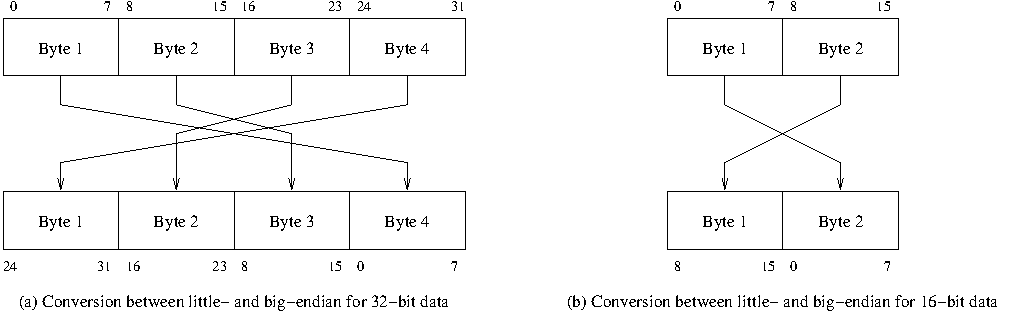
\includegraphics[scale=0.92]{byswpx}
  \end{center}
  \caption{Conversion between big- and little-endian
           \label{fig:cvt-big-ltl-end}}
\end{figure}
%-----------------------------------------------------------------------

It should be noted that the simple byte-swapping above does not work
properly for conversion of other multi-byte structures. For the
purposes of the STL, however, 16-bit structures is the most import
case. For several of the STL modules, the provided test files in
general need to be byte swapped in one or another computer
platform. The documentation and the ``manifesto'' accompaining each
software tool module describe which files, if any, should be
byte-swapped on certain platforms. As default, binary files organized
in 16-bit words are provided in big endian format in the STL
distribution.


%------------------------------------------------------------------------------
\section {Guidelines for software tool development} \hskip 1em \label{UGST-GLs}
%------------------------------------------------------------------------------

The software tools provided by the ITU-T User's Group on Software
Tools are to be used by laboratories with different computers and
A/D-D/A equipment. To make the software accessible to everybody, it
should be highly portable across operating systems and allow for easy
implementation in existing hardware environments.

To achieve this, some simple guidelines were followed in the
development of the tools. The following are the UGST guidelines used to
generate the official and beta releases of the ITU-T Software Tool Library.

\def\labelenumi{\roman{enumi}.}
\def\theenumi{\roman{enumi}}

\begin{enumerate}
\item All software should be written in ANSI C.

\item Features of the language whose representation may create
      side-effects should not be used (e.g. {\tt union}).

\item All variables must be declared and the types used in the
      declarations must be the least platform dependent. For example,
      the keyword {\tt int} must be avoided. Instead \short~ should be
      used for 16-bit integers and {\tt long} should be used for
      32-bit integers.

\item The software should not contain any input or output that may be
      system dependent (e.g. open, read and write file operations).
      Instead, data must be passed to the modules as parameters of
      function calls. This will allow each laboratory to integrate the
      modules with their own application software without changing the
      modules.  Interfaces to various file formats and user
      interaction can optionally be provided as example main
      programs\footnote{\SF Also called {\em ``demonstration
      programs''} in this manual.} that will not be a part of the
      library module and should contain the least possible amount of
      code.

\item Well defined digital signal formats should be used and
      documented for each module to allow the various modules to work
      together.

\item The interface to the file system should be made in a standard way,
      but only within the example programs.

\item The source code should be properly documented, with a standard
      header.

\item Modularity is encouraged in the software design. All modules
      are self-contained, i.e. global definitions should be avoided.

\item Each module should have an attached specification document
      explaining the function and use of the module, the level of
      detail depending on its complexity.

\item The software modules shall be distributed to interested
      laboratories for comments and testing before they are approved
      and included in the ITU-T Software Tools Library, to minimize
      the ocurrence of bugs and to assure conformance with related
      ITU-T Recommendations (when applicable). Two test procedures
      have been devised: compliance and portability.
\end{enumerate}
\def\labelenumi{\arabic{enumi}.}
\def\theenumi{\arabic{enumi}}

The {\em compliance procedure} (or compliance test) is to certify that
a given tool module fully complies with specifications, which should
be carried out by at least one organization other than the proponent
organization (or by a group of organizations, each one checking a
different subset of the specifications, such that all together cover
all the specifications). In order to minimize the probability of
systematic errors, these procedures should be defined by the verifying
organization(s) without input from the tool provider(s).

The {\em portability verification procedure} (or portability test) is
to certify that a given validated tool works on platforms other than
the one(s) where they were generated and validated.  In simple cases
these verification procedures could be just test vectors (e.g. speech
or noise files). It was also pointed out that problems may arise in
Unix platforms, due to the existence of several flavors of Unix
available today (this means that a verification procedure could be
valid in one Unix machine, but not in other).

Portability verification procedures should be provided by the
proponents and shall be run on at least two relevant operating systems
(DOS, UNIX). In the past, procedures for the VMS operating system used
to be required, however this operating system has become less
common. For DOS, the ``pure'' 16-bit mode has become less common, and
16-bit emulation window under a 32-bit version of MS Windows is now
prevalent. These facts affect the choice of compiler.

The following is a list of compilers used to test the portability of
tools in the STL, although not all tools were necessarily tested with
all compilers.

\begin{Descr}{25mm}
\item[\pbox{20mm}{\em HP/c89}] %\rulex{1mm}\\
        This is the {\tt c89} compiler that can be purchased from HP
        for use in HP-UX systems. For the STL, tests with this
        compiler were performed with HP-UX 9.05. \\

\item[\pbox{20mm}{\em HP/gcc}] %\rulex{1mm}\\
        This is the HP-UX port of the {\tt gcc} compiler. The specific
        version may differ from tool to tool. Versions used included
        gcc 2.7.2.2 for HP-UX 9.05 and gcc-2.95.2 for HP-UX 10.20. \\

\item[\pbox{20mm}{\em MSDOS/gcc}]
        This is the MSDOS-6.22 port of the {\tt gcc} compiler version
        2.6.3-DJGPP V1. This is a 32-bit compilation of the code,
        however using a 16-bit interface. Executables are not likely
        to run under Windows MS-DOS emulation window. Needs a run-time
        32-bit extender called {\tt go32.exe}. \\

\item[\pbox{20mm}{\em MSDOS/tcc}]
        This is the Borland Turbo C++ Version 1.00 {\tt tcc}
        compiler. \\

\item[\pbox{20mm}{\em MSDOS/bcc}]
        This is Borland C++ {\tt bcc} compiler. Versions used included
        3.0 and 4.5. \\

\item[\pbox{20mm}{\em Solaris/gcc}]
        This is the {\tt gcc} compiler version 2.95 running under
        Solaris 7, usually in a Sparc platform.\\

\item[\pbox{20mm}{\em SunOS/cc}]
        This is the basic {\tt cc} C compiler bundled in the SunOS
        distribution. For the STL, SunOS version 4.1.3 was used. \\

\item[\pbox{20mm}{\em SunOS/acc}]
        This is the licensed {\tt acc} C compiler sold by Sun
        Microsystems.  For the STL, SunOS version 4.1 was used. \\

\item[\pbox{20mm}{\em Win32/gcc}]
        This is the {\tt gcc} compiler version 2.95 running under
        Windows NT 4 SP 4 and with the CYGWIN Unix emulation
        interface. These executables need either the CYGWIN
        environment or the run-time library cygwin1.dll to run, and
        they are expected to work properly in a DOS emulation window
        under Windows 95/98 as well. This version will not run under
        native MS-DOS. \\

\item[\pbox{20mm}{\em Win32/cl}]
        This is the command-line {\tt cl} version 12.00.8168 C
        compiler of the MS Visual C V.6 SP3 running under the WinNT 4
        SP4 (the executables will also run in Windows
        95/\-98/\-SE/\-Me/\-2000). This version will not run under
        native MS-DOS. \\

\end{Descr}

%\newpage


\section {Software module I/O signal representation} \hskip 1em
%        =====================================================

The idea behind the choice of the convention in this section is that
all software modules within the ITU-T tool library should be
independent building blocks which can easily be combined by connecting
the output of one module to the input of the next module.  With this
characteristic, various systems may be very easily constructed. The
individual software modules must have well-defined interfaces to allow
such simple connections, especially at the I/O level. This convention
is based on the following:

\begin{enumerate}

\item All modules work `from RAM to RAM'. This means that the working
      modules are independent from physical I/O functions which are
      normally machine dependent.  This approach also allows easy
      cascading of modules within one `main' program.

\item All signals at the I/O interfaces of modules are represented in one
      of the following ways:

      \begin{enumerate}
        \item in single or double precision (32 or 64 bit) floating-point
              representation.  The normalized signal is used directly
              ({\em overload point = reference point = 1.0})

        \item in 32 bit 2's complement representation. The normalized signal
              must be multiplied by $\SF 2^{31}$ (i.e. the decimal
              point is just after the MSb, same as for 16 bit
              representation).  If less than 32 bits are required,
              then the signal is left adjusted within the 32 bit
              longword and the LSbs are optionally set to 0.

        \item in 16 bit 2's complement representation, as described in
              section \ref{ovl-point}.  If less than 16 bits are
              required, then the signal is left adjusted
              (left-justified) within the 16 bit words and the LSbs
              are optionally set to 0. If the host machine does not
              provide a format with 16 bit width, then the next
              longer wordlength should be used with the 16 bits right
              adjusted.
      \end{enumerate}

\item Data exchange with a module shall be done directly within the
      calling statement (not by global variables).

\item Data exchange with a module shall be done sample-by-sample
      (FIR-filtering, MNRU, etc.) or frame-by-frame (block oriented
      speech codec, etc.), whichever is more convenient. Larger
      blocks may be formed (e.g. 128 samples at a time) for better
      efficiency, however the block size should be rather small
      (less than 512). The block and its length shall be variables.

\item All modules shall be constructed in a way that infinitely long
      signals may be processed with a reasonable amount of internal storage.
      As an example, the `main' program could read a block of input
      data (e.g., next frame of time signal samples) from the disk,
      call a module or sequence of modules, write the output
      signal (e.g., next frame of coded parameters) back onto disk.
      This process is repeated for all the input data blocks of interest.

\item All modules shall have
      \begin{enumerate}
      \item an initialization part (if necessary) and
      \item a working part
      \end{enumerate}

      The initialization part may be necessary to reset internal
      state variables, define the mode of operation (e.g. MNRU-mode),
      and so on. It is called only once at the beginning or whenever
      a reset to an initial state is needed.

      \NOTE{140mm}{All state variables (if any) must
                be initialized at execution time, not at compile or
                load time.}

      The working part performs the processing itself. It leaves all
      state variables in a well-defined manner for the immediate use
      within the next call. One possible way to do this is to
      introduce a flag-variable within the call statement (e.g.,
      named `Initialize') which is set by the `main' program to '1'
      for initialization and is set to '0' during normal
      operation. In this way, only one function for one module is
      necessary.  Alternatively, a specialized initialization
      routine may be written, to be called before the main
      processing routine of the module. Only one of the approaches
      will be followed in the future. However, both are present in
      the current version of the STL.

\item The RAM allocation shall in principle be split into 'static' and
      'temporary' parts. `Static' means that the contents must be
      saved from call to call, preferrably by means of state variables
      rather than truly static variables\footnote{\SF As a rule, state
      variables should not be defined as truly static ones because
      this may cause side-effects.}. `Temporary' means that the
      contents are not saved between sucessive calls of the module.

\item All modules are separated in clearly and independently defined
      functions, but accompanied by an example `main' program which
      may also include file I/O.
\end{enumerate}


%------------------------------------------------------------------------------
\section {Tool specifications} \hskip 1em
%------------------------------------------------------------------------------

For each tool, there are `Requirements and Objectives' (\ROs)
associated. Each of the \ROs~ has both a general and a specific part.

The general part includes the following\footnote{\SF GL$x$~ refers to
the Guideline number $x$ in section~\ref{UGST-GLs}, e.g., GLiii is the
Guideline iii.}:

\begin{quote}
\begin{enumerate}
 \item Portability among platforms and Operating Systems (DOS, UNIX, and VMS):
        \begin{itemize}
         \item  compilation [GL-i];
         \item  usage of language features that may cause
                  side-effects [GL-ii];
         \item  usage of language  features  that may  be
                  ambiguous among platforms [GL-iii];
         \item  usage of system dependent calls (to access
                  resources such as files, etc.  within the
                  modules) [GL-iv];
        \end{itemize}

 \item Efficiency:
        \begin{itemize}
         \item  use of CPU (i.e., execution speed);
         \item  use of I/O (intensity of access to files, etc.);
         \item  use of memory (physical/virtual);
         \item  code's coverage (verbosity versus laconism);
        \end{itemize}

 \item Documentation:
        \begin{itemize}
         \item  Self-documentation (e.g., comments, variables and structure
                  resembling ITU-T Recommendations, etc.)[GL-vii];
         \item  Separate documentation (clarity, objectivity, etc.)[GL-ix];
        \end{itemize}

  \item Modularity [GL-viii]

  \item Fixed- versus floating-point implementations;
\end{enumerate}
\end{quote}


Following are descriptions of each of the General \ROs. Full
description of the \ROs~ can be found in \cite[Annex 4]{COM-XV-R-73-E}.

{\em General performance specification} refers to the
document that specifies the tool in question, e.g. an ITU-T
Recommendation or ANSI or ETSI standard.

{\em Portability} addresses several points related to the tool's
capacity of working on several platforms: {\em Compilation and
linkage} refers to the necessity of changes in the source code to make
a tool compile without any modification in a given environment.  It
was identified that the operating systems of most interest are DOS and
Unix (both BSD and System V). {\em Side-effectable features} are those
that, if used in a program, when changing one parameter, may cause
other(s) to be changed implicitly. {\em Ambiguous features} are those
that, due to the flexibility left in the C language specification, are
implemented in different ways for different platforms. For example,
{\tt int} in C is 32-bit wide in VAX-C and Unix workstations, but is
16-bit wide for most compilers available on MS-DOS
(Turbo-C/MS-C). {\em System-dependent calls} are calls that are
restricted to or are implementation of features of a particular
platform, to make better use of that particular computer architecture.

{\em Efficiency} is related to how the computer's resources
are used in terms of CPU, I/O and memory allocation, that may be a
burden and prevent the usage in some systems, either by lack of
resources or length of time needed for execution. Efficiency also
includes {\em code's coverage}, expressing how frequently code is
accessed.

{\em Documentation} refers to how to describe the tool. {\em
Self-documentation} is the documentation present in the program itself
to assure that the code clearly describes the algorithm
implemented, to provide compilation and linkage instructions, as well as
to report known bugs, etc. A {\em separate document} will
be mandatory when no written description of the algorithm is available,
or when the written documents that specify the tool are too general.

{\em Modularity degree} is the degree of isolation that a particular
tool has. From UGST Guidelines, all tools must be modular, i.e.,
self-contained blocks; nonetheless, tools may make use of system
resources other than memory and CPU.

{\em Arithmetic} is the number representation specification, either in
fixed (2's complement, 1's complement, etc.) or floating point. Here,
``fixed-point'' shall always be understood as 2's complement
representation, except where otherwise indicated.
